\newpage
\section{Realisering og test}
\label{realiseringOgTest}

%Her kan du skrive om realisering og test
For å realisere systemet i Figur \ref{fig:prinsipp_ulinært} ble det brukt et ulineært system som er vist i Figur \ref{fig:transistor}. Det ulineære systemet er basert på en transistor forsterker og en LC ocillator. LC ocillatoren som er koblet på utgangen av transistor forsterkeren er for å skape en frekvens som er dobbelt så høy som den orginale frekvensen og utregnineres med formelen $f = \frac{1}{2\pi\sqrt{LC}}$, hvor $f=3.8$kHz$=x_2$. Spolen somble benyttet hadde verdien $L_1=10\mu$H og tilhørende kondensatorverdi ble da $C_1=180\mu$F. Grunnen til å benytte seg av noe sånt er fordi denne kretsen vil forsterke den inkommende signalet og i tillegg generere mye kraftigere signal på den ønskede frekvensen så et mindre nøyaktig filter kan brukes. 

\begin{figure}[!h]
    \centering  
    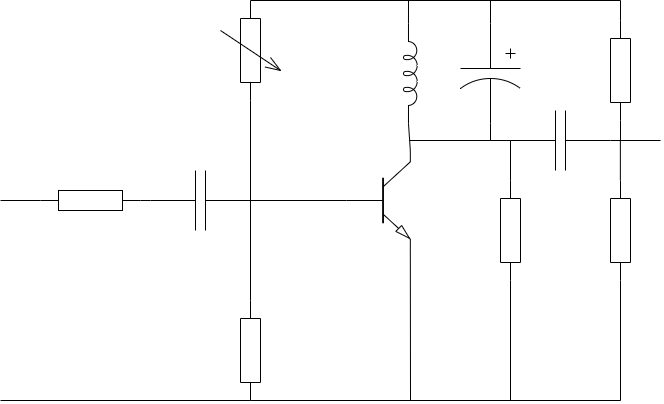
\includegraphics[width=0.8\textwidth]{Bilder/transistor.drawio.png}
    \caption{Transistor forsterker og LC ocillator}
    \label{fig:transistor}
\end{figure}

En op-amp er så brukt for å buffre systemet før det går inn i båndpass filteret som er vist i Figur \ref{fig:bandpass}. Båndpass filteret er basert på en LC krets som er koblet i serie med en motstand. Denne kretsen er designet for å isolere ut den ønskede frekvensen og bode diagrammet er vist i figur \ref{fig:bode_diagram}. Knekkfrevnsen ble regnet ut med samme formel som over og er $f = \frac{1}{2\pi\sqrt{LC}}$ med en spole på $L=110$mH og condensatoren endte opp på $C=16$nF.

\begin{figure}[!h]
    \centering  
    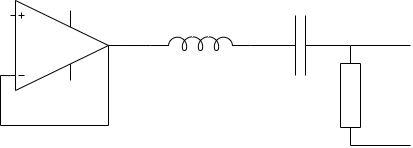
\includegraphics[width=0.8\textwidth]{Bilder/bandpass.drawio.png}
    \caption{Båndpass filter}
    \label{fig:bandpass}
\end{figure}

\begin{figure}[!h]
\centering
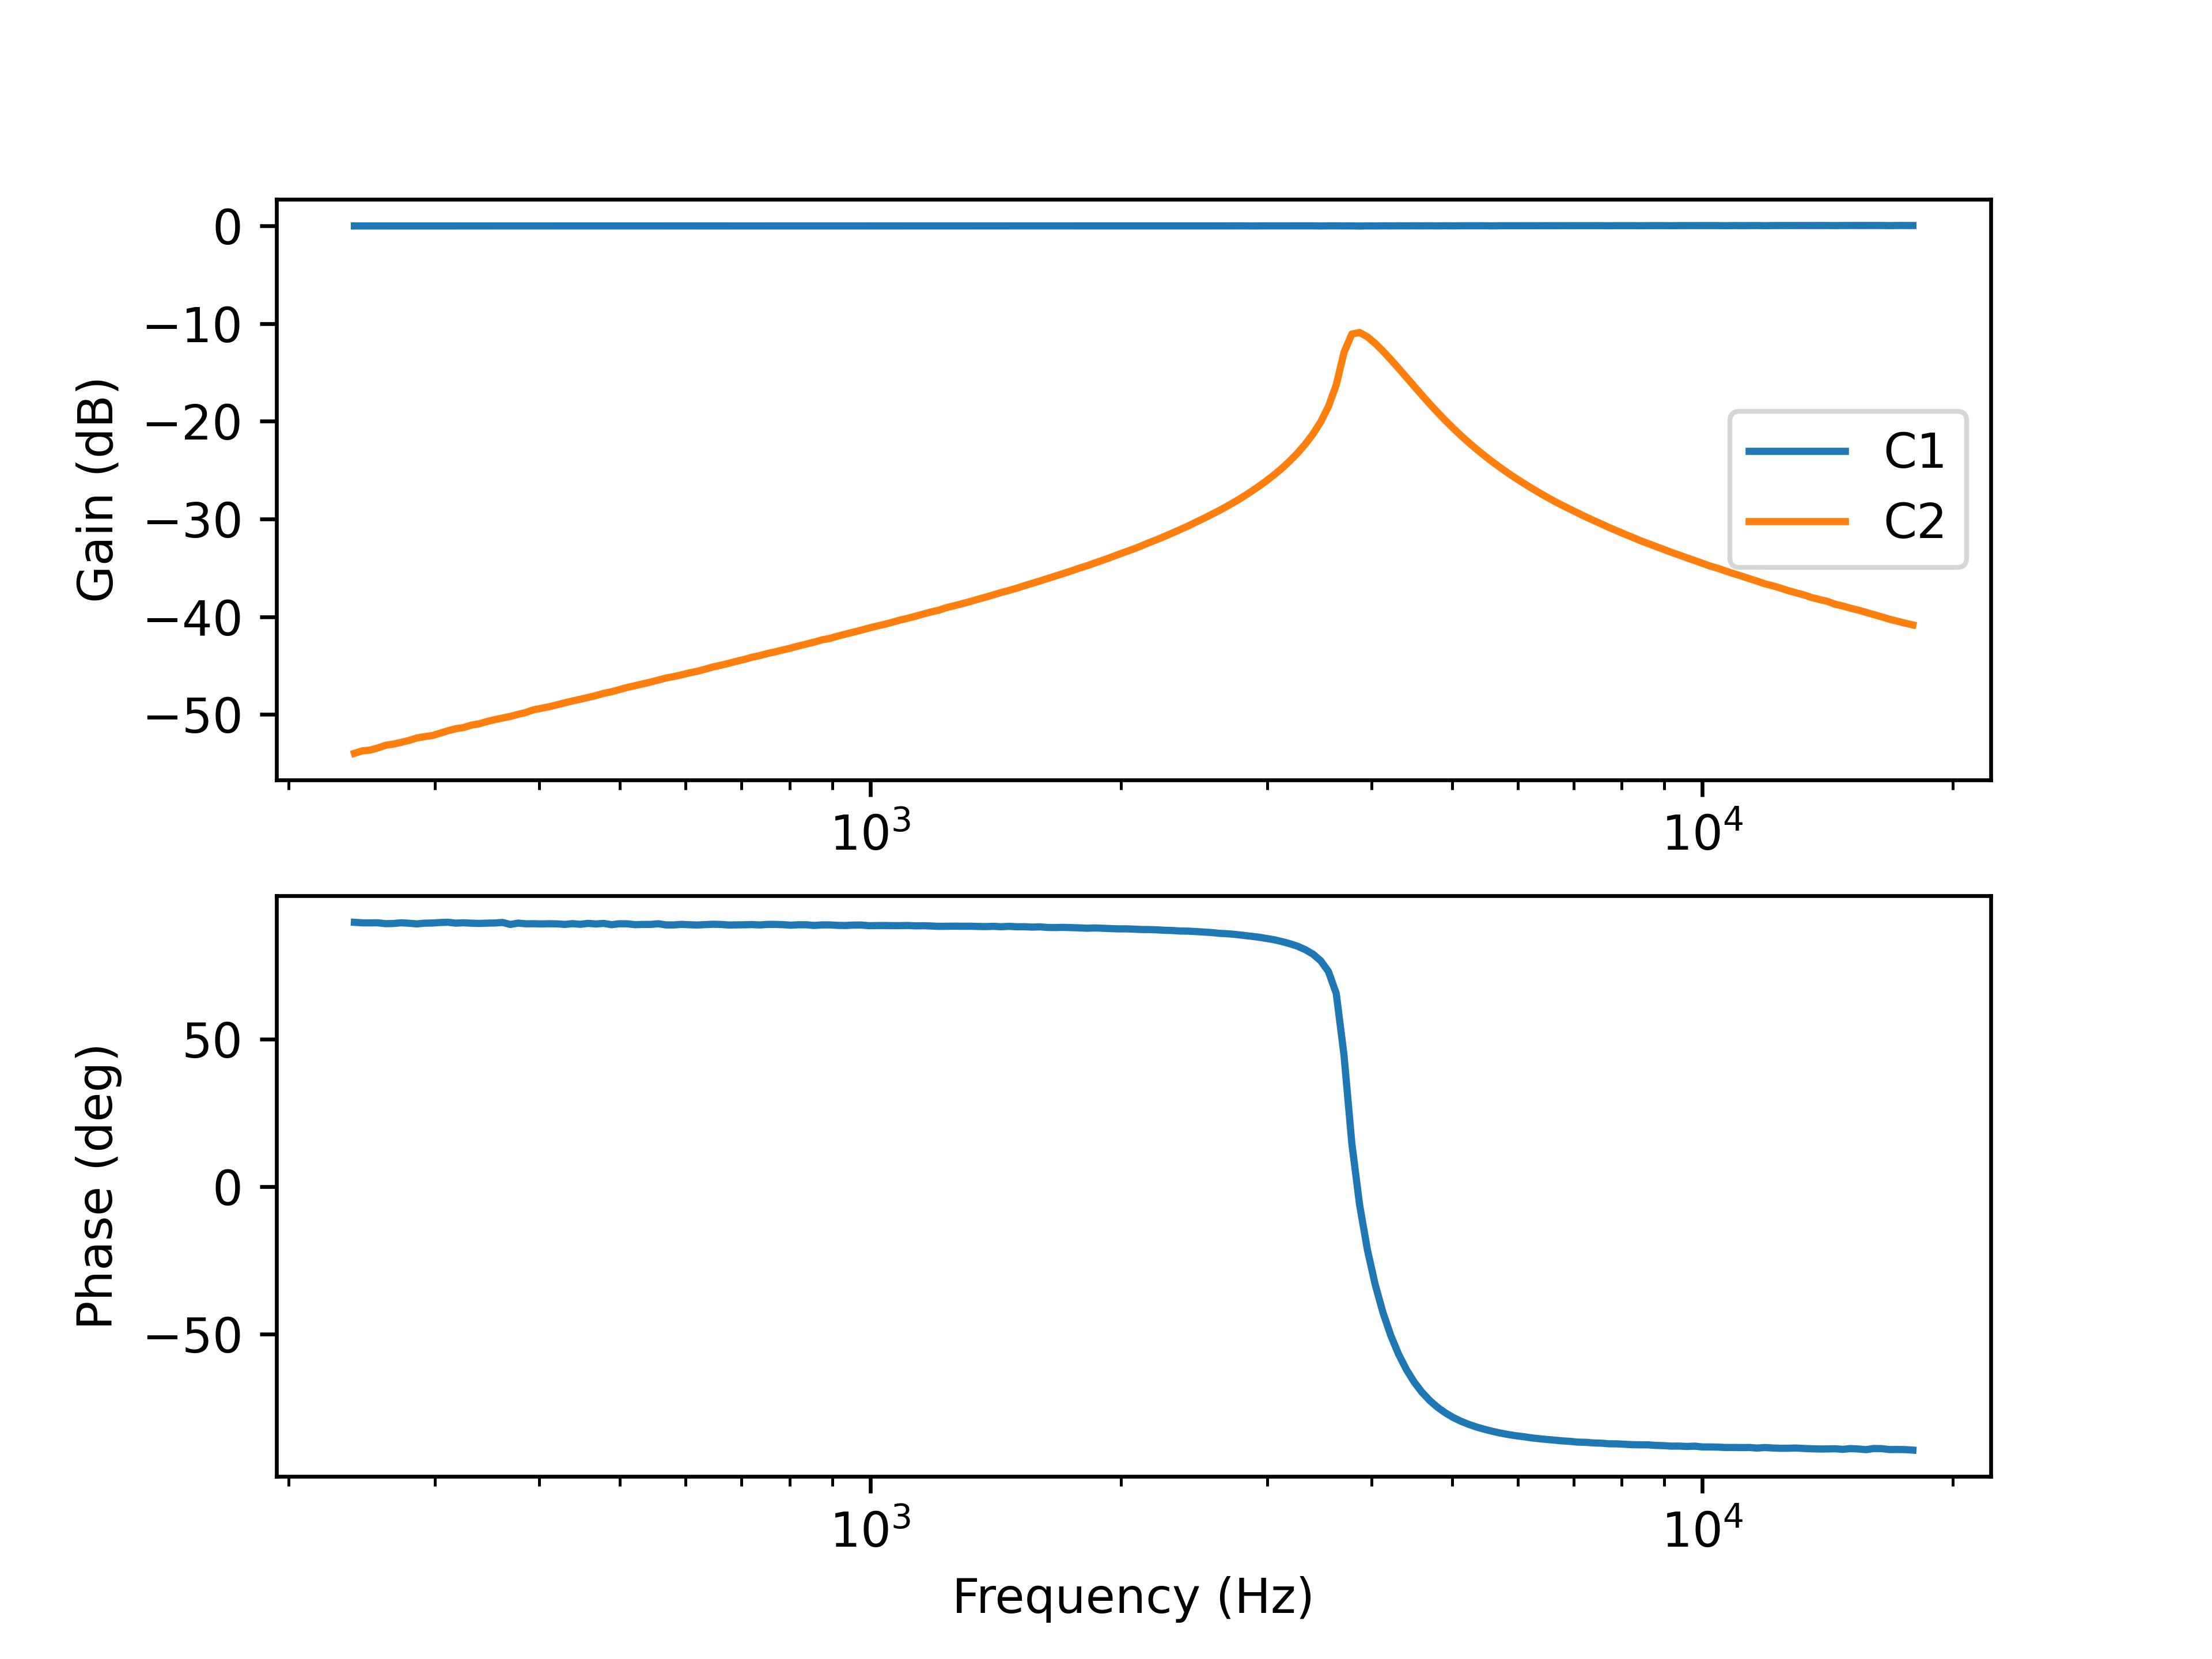
\includegraphics[width=0.8\textwidth]{Bilder/bode.png}
\caption{Bode diagram for båndpass filteret}
\label{fig:bode_diagram}
\end{figure}

Et kretsskjema av det totale systemet er vist i figur \ref{fig:realisert_system_skjema}.

\begin{figure}[!h]
\centering
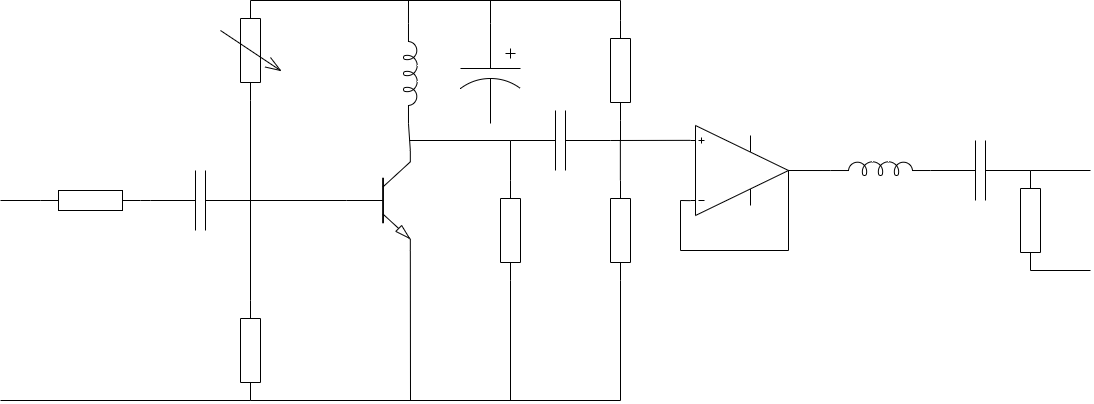
\includegraphics[width=0.8\textwidth]{Bilder/Realisert_system_skjema.drawio.png}
\caption{Realisering av systemet}
\label{fig:realisert_system_skjema}
\end{figure}


For realisering av systemet i Figur \ref{fig:realisert_system_skjema}, ble det brukt et sinussignal på $f = 1.9$kHz. Som vi kan lese av plottet i figur \ref{fig:spectrum} så er ikke den orginal frekvensen borte men senket med ca 50dB. Dette er fordi det ikke er mulig å få en perfekt frekvensdobling med et ulineært system. Vi har derimot fått en frekvensdobling på ca 3.8kHz som er ca 40dB høyere enn det orginale signalet på samme frekvens. 

\begin{figure}[!h]
\centering
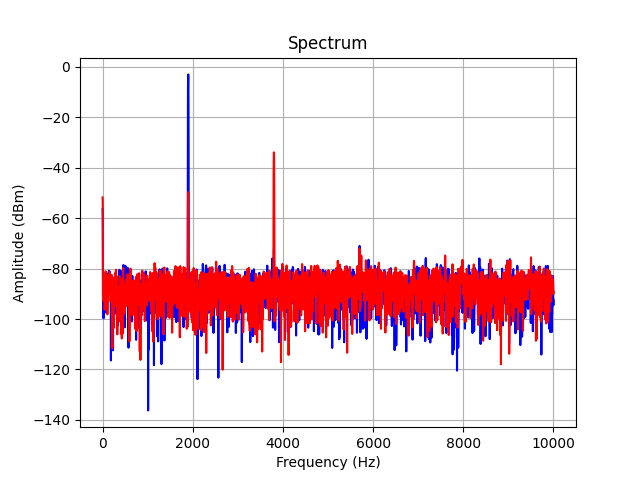
\includegraphics[width=0.8\textwidth]{Bilder/Spectrum.png}
\caption{Spectrum av signalet}
\label{fig:spectrum}
\end{figure}

Et bilde av oppkoblet krets vises i figur \ref{fig:realisert_system}.

\begin{figure}[!h]
\centering
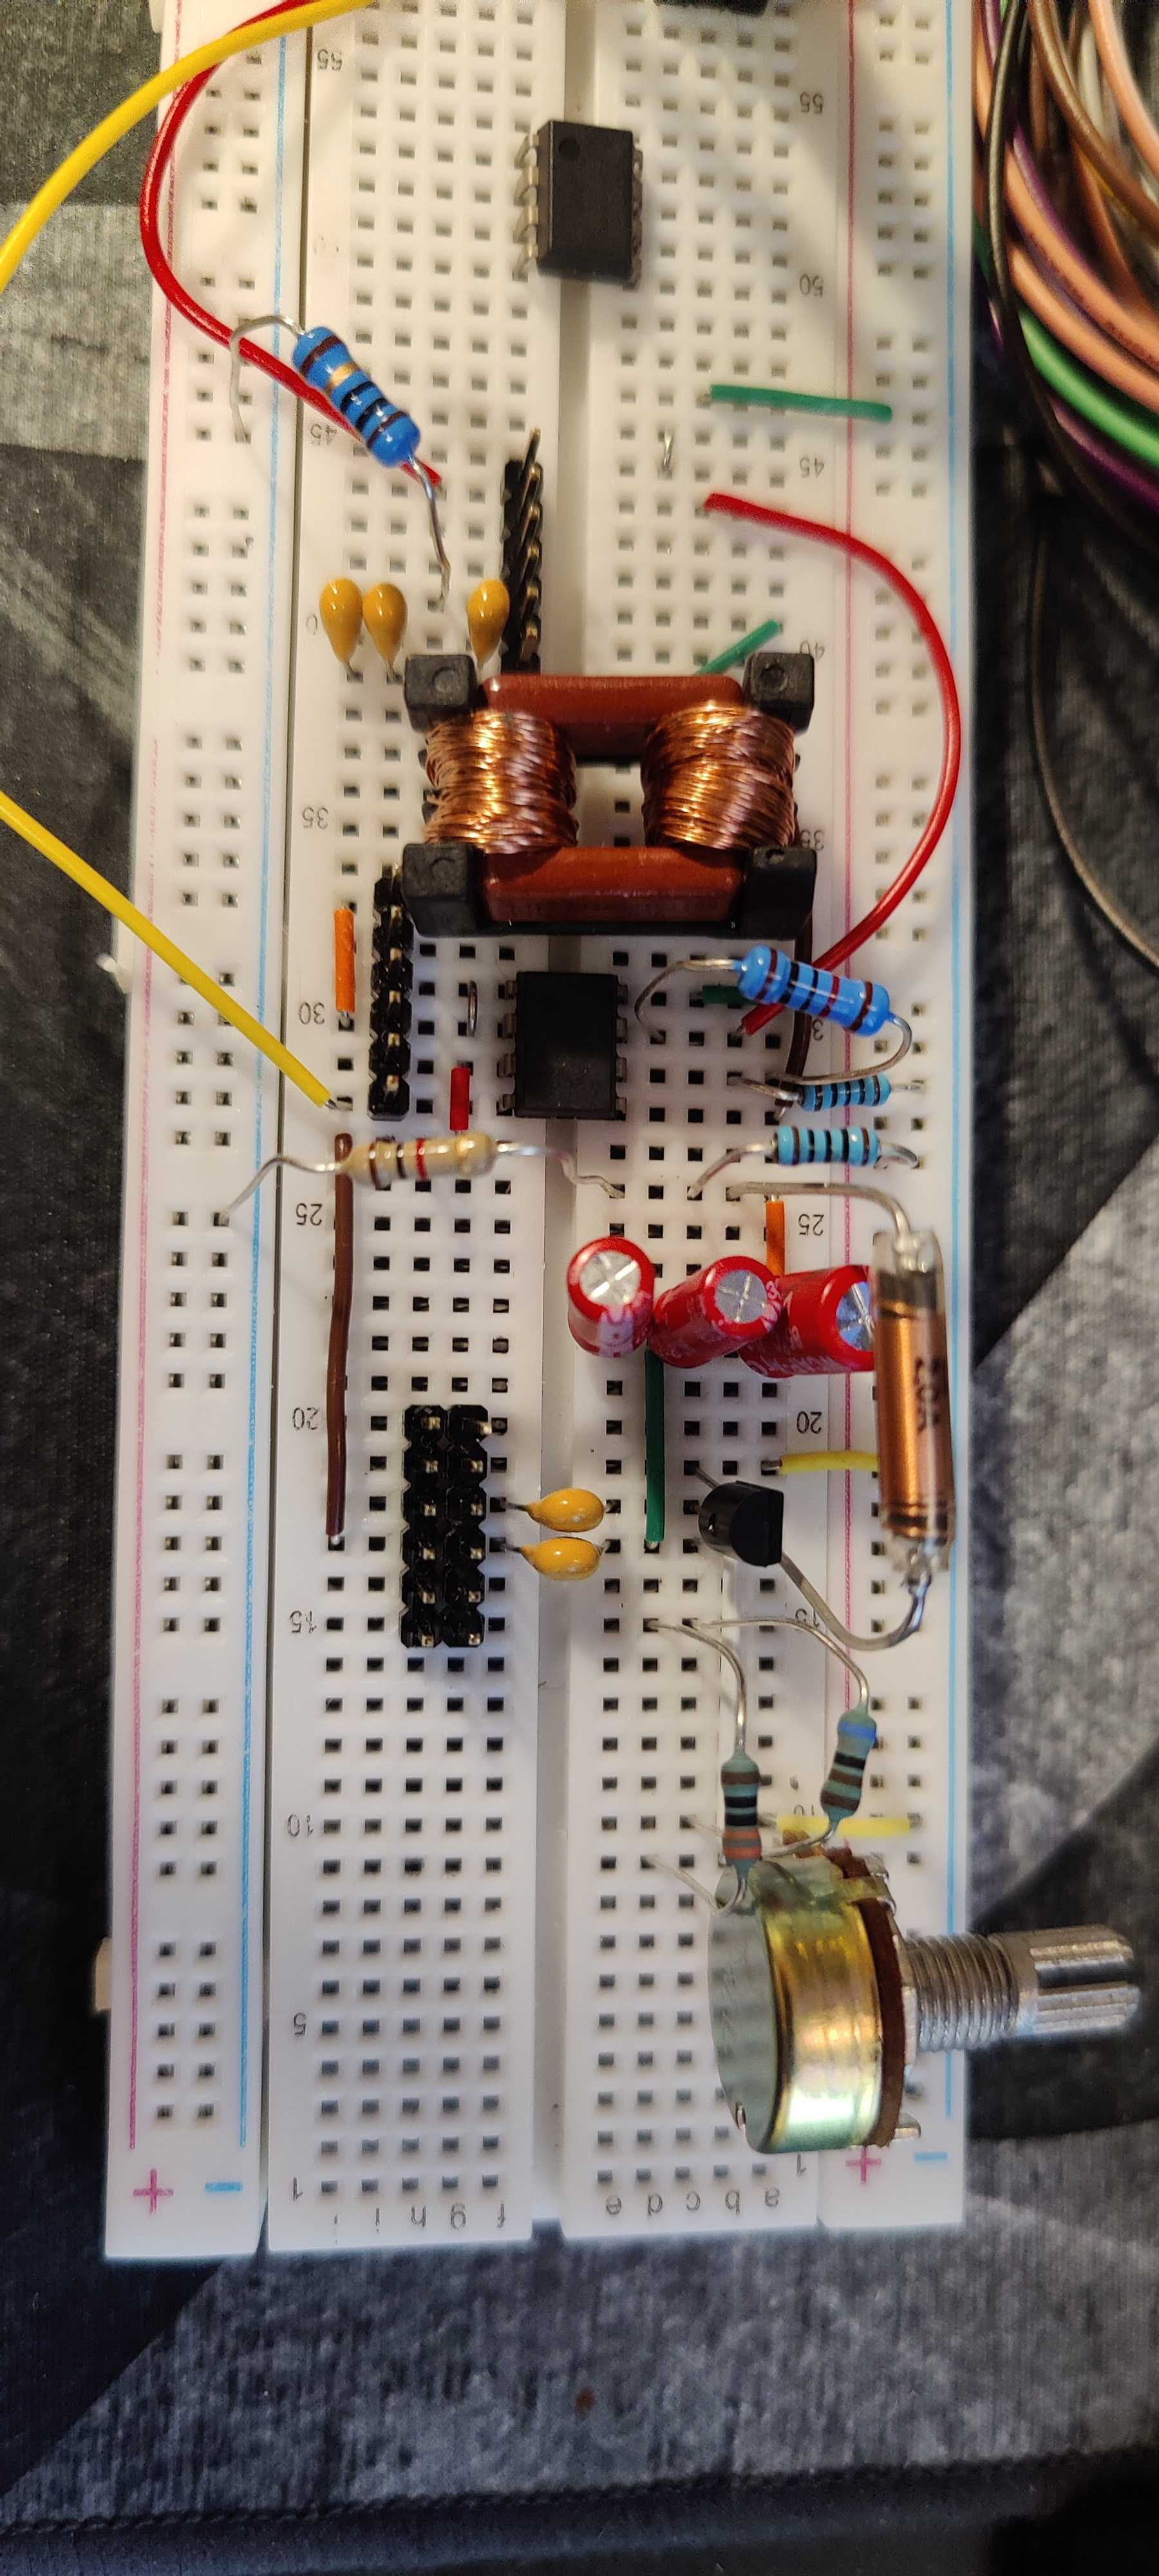
\includegraphics[angle=90,width=0.9\textwidth]{Bilder/Realisert_system.jpg}
\caption{Realisert system}
\label{fig:realisert_system}
\end{figure}